\chapter{Symmetry and SAT}\label{chap:symmetryinsat}

%This chapter presents the computation and usage of symmetry in SAT problems.


The group of permutations of $\Vars$ (i.e. bijections from $\Vars$ to $\Vars$) is noted
$\Group(\Vars)$. The group $\Group(\Vars)$ naturally acts on the set of literals: for $g
\in \Group(\Vars)$ and a literal $\ell \in \Lits $, $g.\ell = g(\ell)$ if $\ell$ is a
positive literal, $g.\ell = \neg g(\neg \ell)$ if $\ell$ is a negative literal.
The group $\Group(\Vars)$ also acts on (partial) assignments of $\Vars$ as follows: for
$g \in \Group(\Vars)$, $\alpha \in \Assignments(\Vars)$, $g.\alpha = \{ g.\ell ~|~ \ell \in \alpha \}$. Let $\varphi$ be a formula, and $g \in \Group(\Vars)$. We say that $g\in \Group(\Vars)$ is a
symmetry of $ \varphi$ if for every \emph{complete} assignment $\alpha$, $\alpha
\models \varphi$ if and only if $g.\alpha \models \varphi$. The set of symmetries
of $\varphi$ is noted $S(\varphi) \subseteq \Group(\Vars)$.



The previous mathematical definitions of group theory is applied to the CNF formula.
So, the group of permutations of $\Vars$ (i.e. bijections from $\Vars$ to $\Vars$) is noted
$\Group(\Vars)$. We say that $g\in \Group(\Vars)$ is a symmetry of $ \varphi$ if following conditions holds:
\vspace{-1em}
\begin{itemize}[topsep=1em]
	\item permutation fixes the formula, $g.\varphi =  \varphi$ 
	\item $g$  commutes with the negation: $g.\neg l  = \neg g.l$
\end{itemize}

The set of symmetries of $\varphi$ is noted $S(\varphi) \subseteq \Group(\Vars)$.
The sets of symmetries of a formula $\varphi$ preserves the satisfaction,
for every \emph{complete} assignment $\alpha$, 
$\alpha \models \varphi \leftrightarrow g.\alpha. \models \varphi$ for $g \in S(\varphi)$.
The group $S(\varphi)$ also acts on (partial) assignments of $\Vars$ as follows: for
$g \in S(\varphi)$, $\alpha \in \Assignments(\Vars)$, $g.\alpha = \{ g.\ell ~|~ \ell \in \alpha \}$,
and acts also on clauses as follow g.$\omega$ = $\{g.l ~|~ l \in \omega \}$.


The next section presents how to compute the set of \emph{generators} of a given formula.

\section{Symmetry detection in SAT}

For the detection of symmetries in SAT, we fist introduce the graph automorphism notion.
Given a colored graph $G = (V, E, \gamma)$, with vertex set $V \in  [1, n] $, edge set E and
$\gamma$ a function that apply a mapping : $V \rightarrow C$ where C is a set of \emph{colors}.
An automorphism of G is a permutation from its vertices $g :V \rightarrow V$ 
such that:
\begin{itemize}
	\item $\forall (u, v) \in E \implies (g.u, g.v) \in E$
	\item $\forall v \in V, \gamma(v) = \gamma(g.v)$
\end{itemize}

The graph automorphism problem is to find if a given graph has a non trivial permutation group. 
The computational complexity of this algorithm is conjectured to be strictly between P and NP.
Several tools exists to tackle this problem like \saucy~\cite{katebi2010symmetry},
\bliss~\cite{JunttilaKaski:ALENEX2007}, \nauty~\cite{mckay2003nauty}, etc.



There exists different ways to encode a SAT problems,
which leads to different symmetries in these problem.
When a symmetry depends on the structure of the problem, we say \emph{syntactic} symmetries. 
In contrast, symmetries were \emph{semantic}, when it is not inherent to the encoding.
To find symmetries in SAT problem, the formula is transformed into colored graph
and an automorphism tool is applied onto. Specifically, given a formula $\varphi$ with
$m$ clauses over $n$ variables, the graph is constructed as follows:
\begin{itemize}
	\item \emph{clause nodes}: represent each of the $m$ clauses by a node with color 0;
	\item \emph{literals nodes}: represent each of the $l$ literals by a node with color 1;
	\item \emph{clauses edges}: connect each clause node to the node of the literals that appear in clause;
	\item \emph{boolean consistency edges}: connect each pair of literals that correspond to the same variables.
\end{itemize}


\begin{figure}[h!]
	\begin{minipage}[c]{.2\textwidth}
		\lstinputlisting[numbers=none]{cnfs/battleship-3-4-unsat.cnf}
	\end{minipage}
	\begin{minipage}[l]{.75\textwidth}
		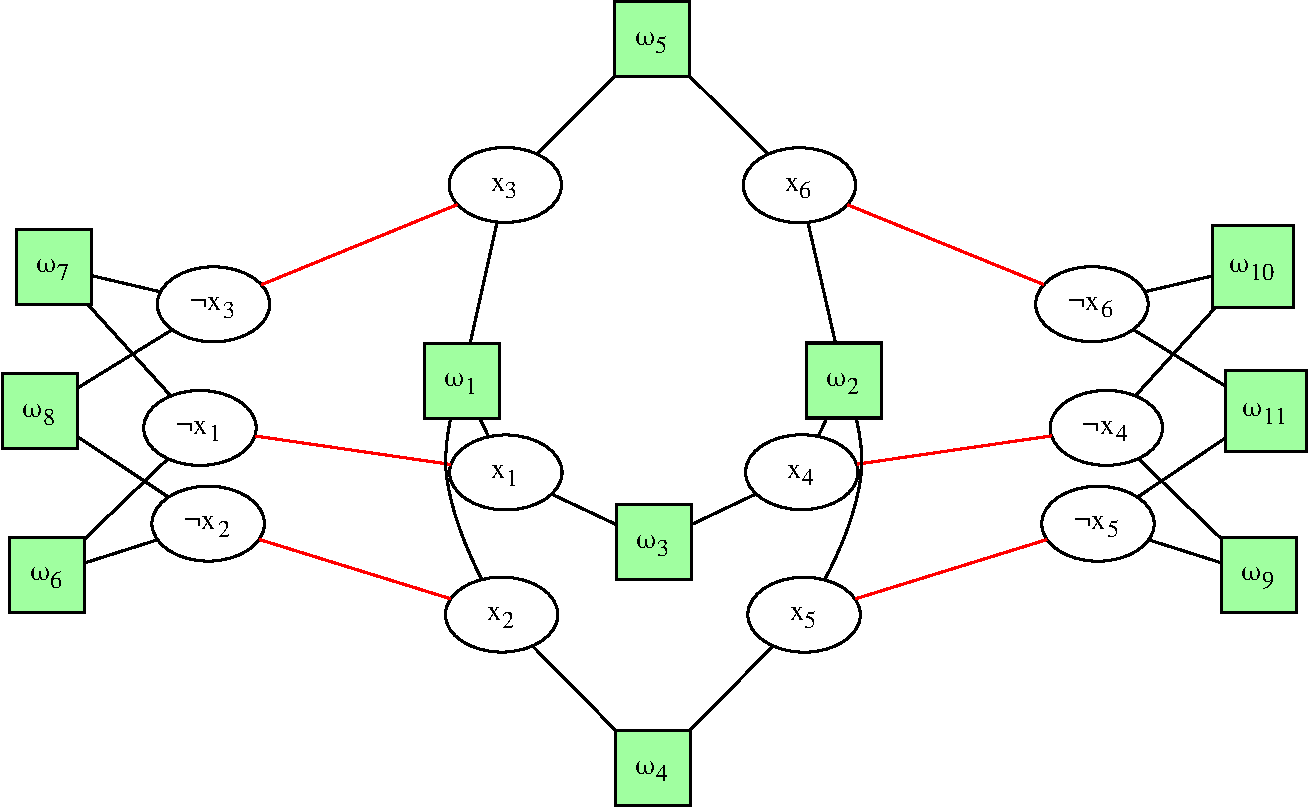
\includegraphics[width=4.3in]{cnfs/graph_cnf_no_opt-crop}
	\end{minipage}
\caption{Example of constructed symmetry graph for a given CNF}
\end{figure}

\hakan{Explication du graph + informations num nodes num edges. Probleme reel battleship
}

The battleship problems place one  ship of size *** and two ships of size* in grid 3x4 \\
1  2  3\\
4  5  6\\
7  8  9\\
10 11 12\\

one ship per row.\\

Produced graph contains 12 * 2 = 24  + 21 = 45 nodes and 24 + 36 = 60 edges 

\clearpage

An optimization of this graph is possible with the usage of binary clauses i.e. a clause with only two literals.
The clause node can be omitted and we connect the two literals. As we cannot distinguish between the optimized edge 
and boolean consistency edges, we must check if the produced permutations are spurious. 
To do so, as we ensure the permutation commutes with the negation it suffice to check:
$\forall x \in \support(g), g.\neg x = \neg g.x$.
Roughly speaking, we check if the image of the negation of $x$ is equals to the negation of the image of $x$, for each element $x$ in the support of the permutation.
This optimization allows to compute symmetries of the problem more efficiently.
In the previous example, the graph has deleted 12 nodes and 12 edges. More generally,
the graph removes as many nodes and edges as binary clauses on the formula.

\begin{figure}[h]
	\begin{minipage}[c]{.2\textwidth}
		\lstinputlisting[numbers=none]{cnfs/battleship-3-4-unsat.cnf}
	\end{minipage}
	\begin{minipage}[l]{.75\textwidth}
		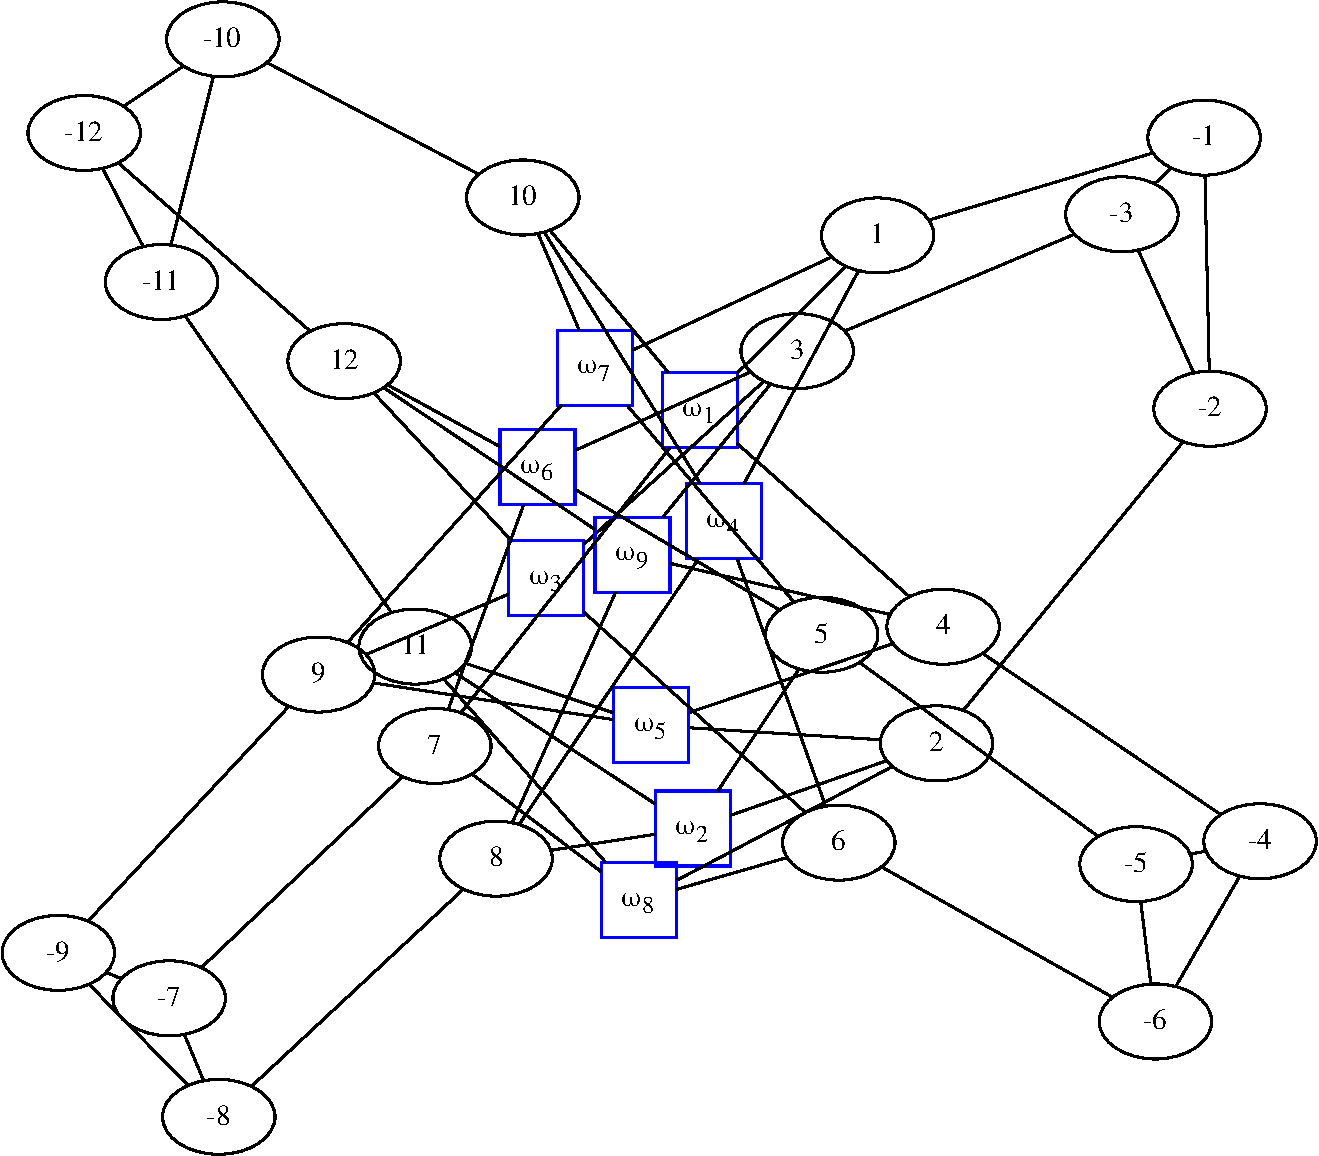
\includegraphics[width=4.3in]{cnfs/graph_cnf_opt-crop}
	\end{minipage}
	\caption{Example of constructed symmetry graph for a given CNF}
\end{figure}


%\hakan{optimisation du graph}\\
%\hakan{creation d'un probleme fil conducteur and utilisation de celui dans chaque partie, du calcul des symétries
%jusqu'au SBP}\\

When these graph is given to an automorphism tool like \bliss, the following \emph{generators} are 
obtained:
\begin{itemize}[topsep=0em]
\item $g_0$: (2 3)(5 6)(8 9)(11 12)(-2 -3)(-5 -6)(-8 -9)(-11 -12)
\item $g_1$: (4 5 6)(7 9 8)(-4 -5 -6)(-7 -9 -8)
\item $g_2$: (4 7)(5 8)(6 9)(-4 -7)(-5 -8)(-6 -9)
\item $g_3$: (1 2)(5 6)(7 9)(10 11)(-1 -2)(-5 -6)(-7 -9)(-10 -11)
\item $g_4$: (1 10)(2 11)(3 12)(-1 -10)(-2 -11)(-3 -12)
\end{itemize}


The visualization of the orbits of literals on the problem could be seen in figure~\ref{fig:orbits}, where each node represents a literal. Two literals are 
linked with an arc if it exists a permutation that maps the literal to the second one.
By definition of the orbits, each literal belongs to a strongly connected components (SCC).

 \begin{figure}[h]
 	\centering
 		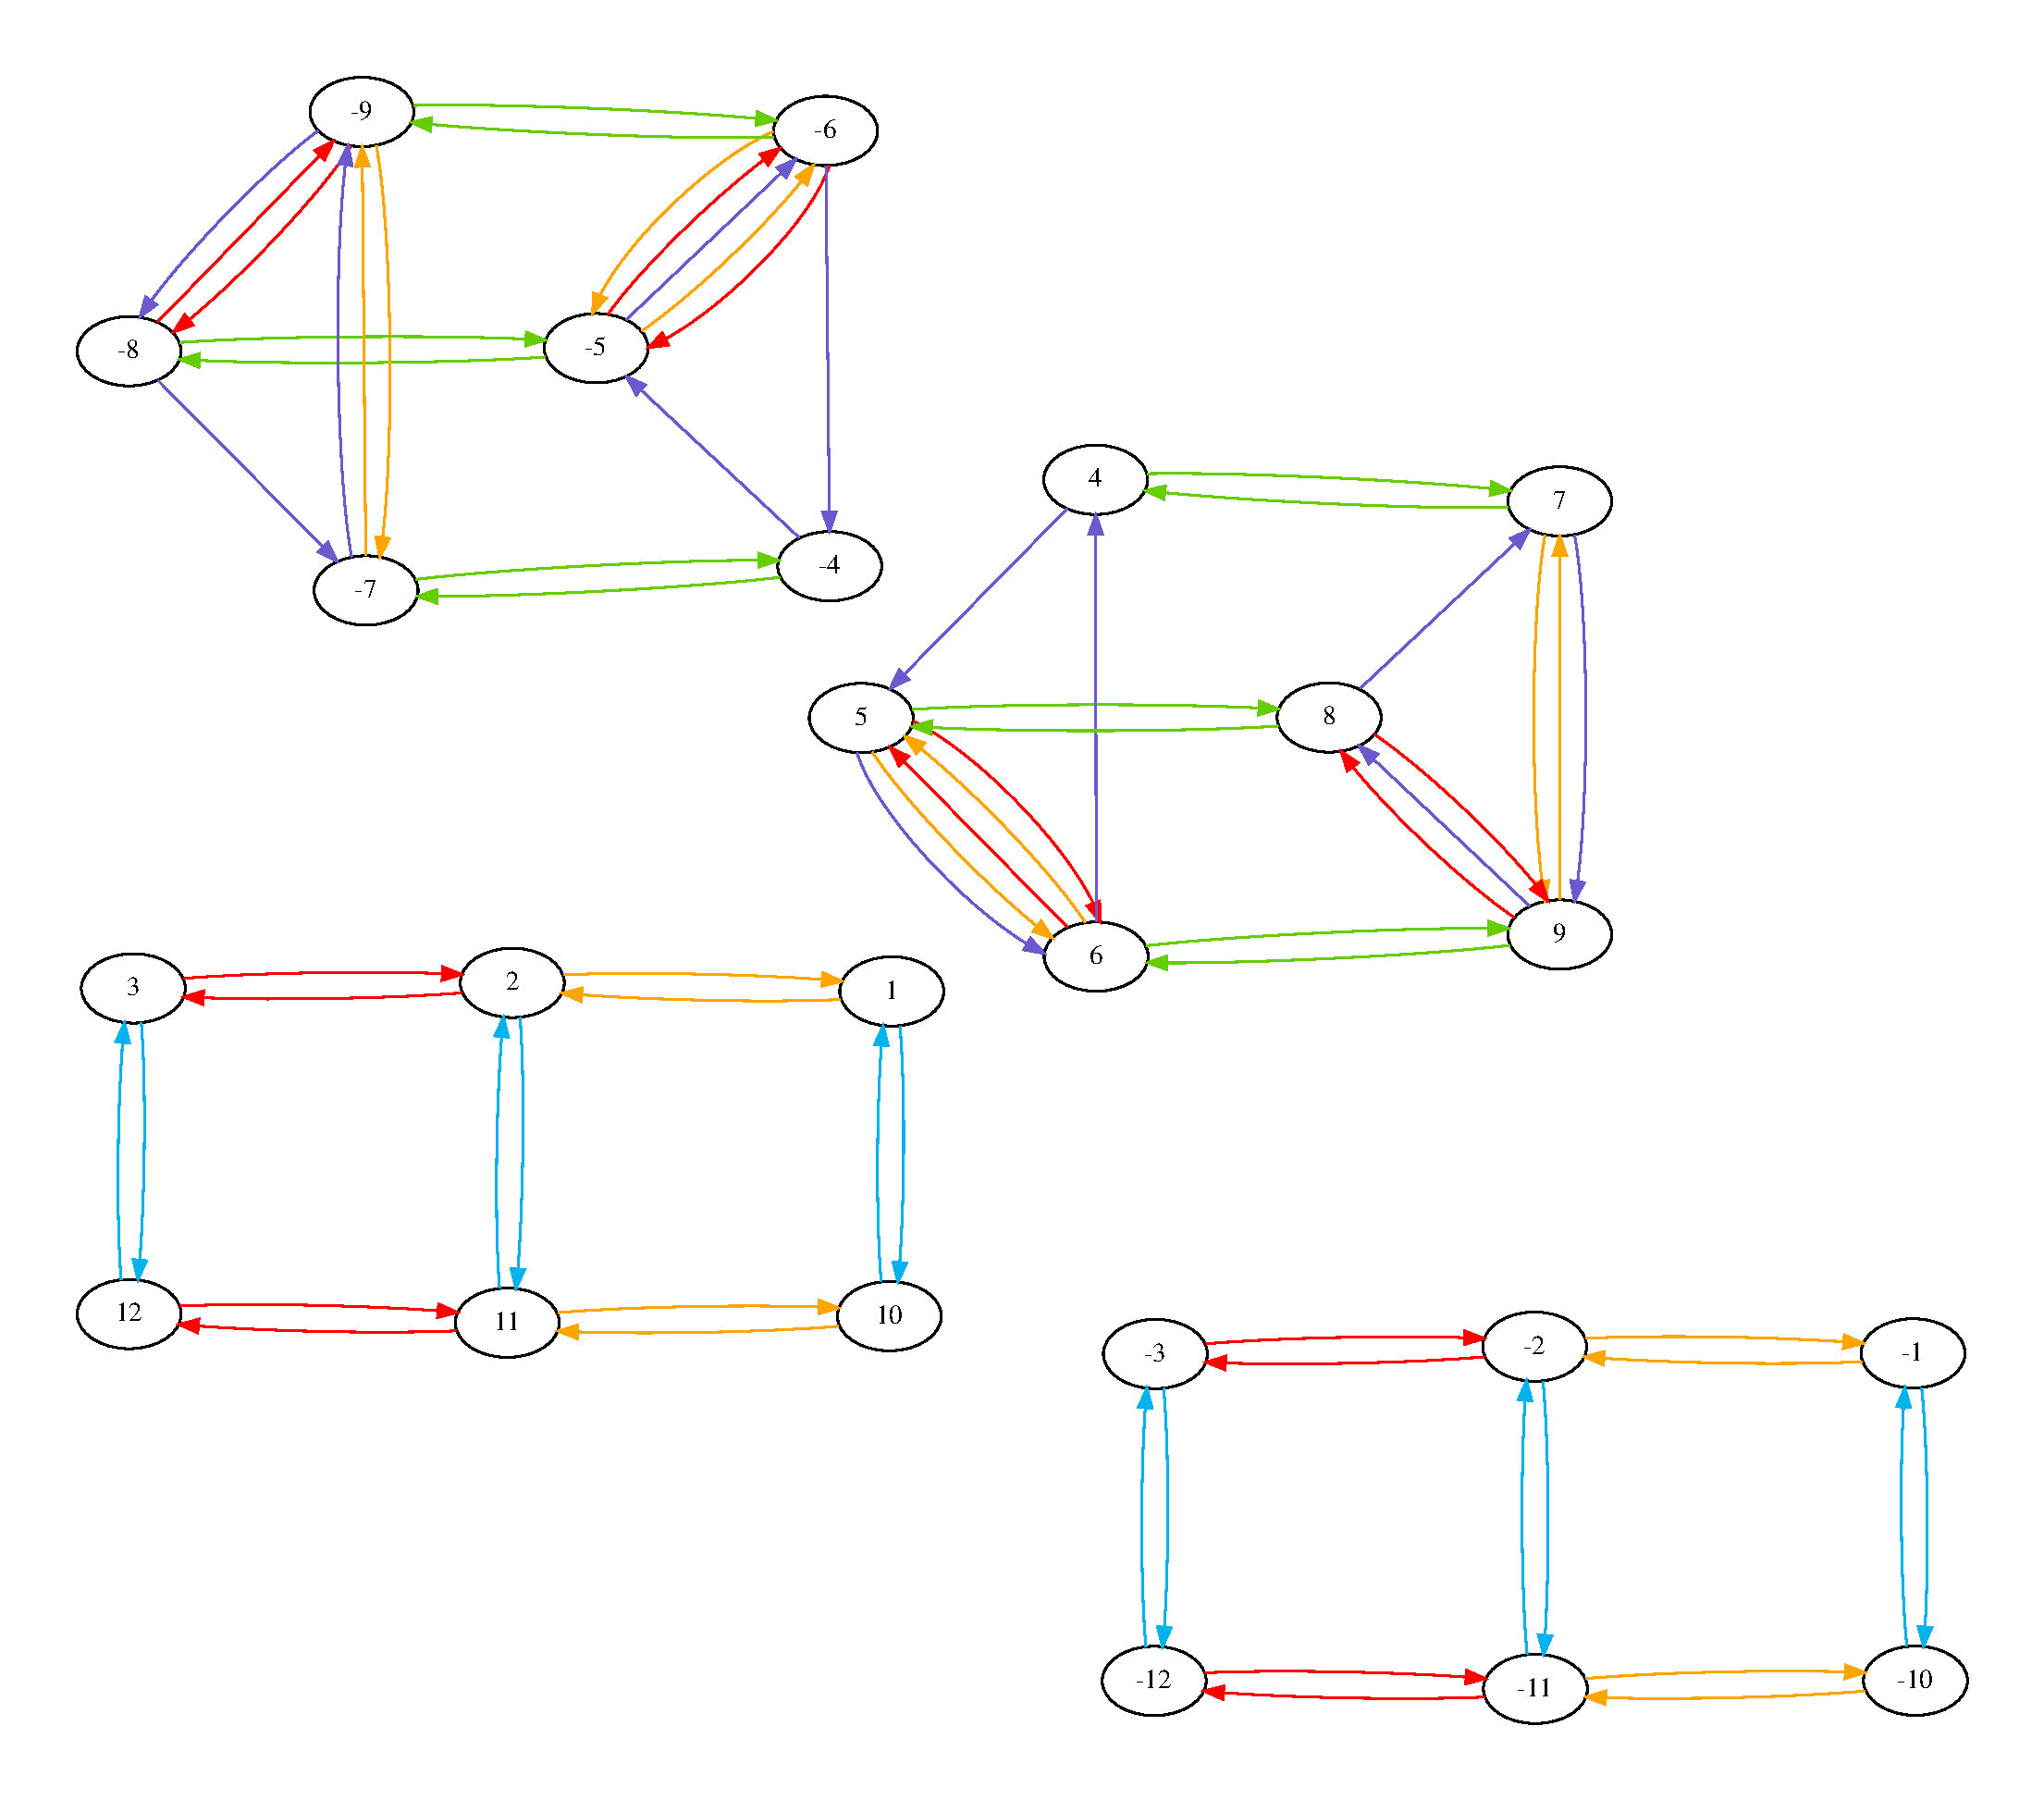
\includegraphics[width=\textwidth]{cnfs/orbits}
 	\caption{Orbits}
 	\label{fig:orbits}
 \end{figure}



\section{Usage of symmetries}

\emph{Symmetry breaking} aims at eliminating symmetry, either
by \emph{statically} posting symmetry breaking constraints that invalidate symmetric
assignments, or by altering the search space \emph{dynamically} to avoid symmetric search paths.


In order to exploit the symmetry properties of a SAT problem, we need to
introduce an ordering relation between the assignments.

\begin{definition}[Assignments ordering]
	\label{def:assignment_ordering}
	We assume a total order, $\prec$, on $\Vars$.  Given two assignments $(\alpha,\beta) \in \Assignments(\Vars)^2 $, 
	we say that $\alpha$ is strictly smaller than $\beta$, noted $\alpha < \beta$, if there exists a variable $v \in \Vars$
	such that:
	\begin{itemize}
		\item for all $v' \prec v$, either $v' \in \alpha \cap \beta$ or $\neg v' \in \alpha \cap
		\beta$.
		\item $\neg v \in \alpha$ and $v \in \beta$.\footnote{We could have chosen as well $v \in \alpha$ and $\neg v \in \beta$ without loss of generality.}
	\end{itemize}
\end{definition}

Note that $<$ coincides with the lexicographical order on \emph{complete}
assignments. Furthermore, the $<$ relation is monotonic as expressed in the following proposition:

\begin{proposition}[Monotonicity of assignments ordering]
	\label{prop:monocity_assignments_ordering}
	Let  $(\alpha,\alpha',\beta,\beta') \in \Assignments(\Vars)^4 $ be four assignments.
	$$\text{If}~\alpha \subseteq \alpha'~\text{and}~\beta \subseteq \beta',~\text{then}~\alpha < \beta \implies \alpha' < \beta'$$
\end{proposition}

\begin{proof}
	The proposition follows on directly from Definition \ref{def:assignment_ordering}.
\end{proof}


Let $\varphi$ a formula, and $G$ the group from the formula.
The \emph{orbit of $\alpha$ under $G$} (or
simply the \emph{orbit of $\alpha$} when $G$ is clear from the context) is the set
$ [\alpha]_G=\{ g.\alpha \mid g \in G \}$. The lexicographic leader
(\textit{lex-leader} for short) of an orbit $[\alpha]_G$ is defined by
$min_<([\alpha]_G)$. This \textit{lex-leader} is unique because the lexicographic
order is a total order.
The optimal approach to solve a symmetric SAT problem would be to explore
only one assignment per orbit (for instance each lex-leader). However, finding the
lex-leader of an orbit is computationally hard~\cite{Luks2004}. To avoid exploring 
symmetry search space, \emph{symmetry breaking predicates} are added to the formula.
These constraints are true only for the \emph{lex-leader} \cite{crawford1996symmetry}.




%\begin{definition}[Stabilizer of permutation]
%	Let two permutation $g_1$ and $g_2$, we say that $g_1$  stabilize $g_2$
%	$$\text{If}~ \support(g_1) \cap \support(g_2) = \emptyset$$
%\end{definition}


\begin{theorem}[Satisfiability preservation SBPs]
	\label{theorem:satisfiability_preservation_SBPs}
	Let $\varphi$ be a formula and $\psi$ the computed \textit{SBPs} for the set of
	symmetries $S(\varphi)$
	
	$$\varphi~and ~\varphi \wedge \psi \text{ are equi-satisfiable}.$$
\end{theorem}

\begin{proof}
	If $\varphi \wedge \psi$ is SAT then $\varphi$ is trivially SAT. If
	$\varphi$ is SAT, then there is some assignment $\beta$ that satisfies $\varphi$.
	Without loss of generality, $\beta$ can be chosen to be the lex-leader of its
	orbit under $S(\varphi)$. Thus, $g$ does not contradict $\beta$, which implies that
	$\beta \models \psi$.
\end{proof}

 
\hakan{Refaire la figure avec plus de point}
\begin{figure}
	\centering
%	\includegraphics[width=2in]{fig/assignment-lex-leader}
	\begin{tikzpicture}
    \tikzstyle{point}=[circle,draw,thick,fill=black,scale=0.2]
	\tikzstyle{point+}=[circle,draw=red,thick,scale=0.4]


\begin{scope}
\node[ellipse, draw, minimum width=4cm, minimum height=2cm] (c1) at (2.5,0){};
	\clip (2.5, 0) ellipse (2 and 1);
	\node[point+] (p2) at (1, 0.3){};
	\pgfmathsetseed{281}
	\foreach \p in {1,...,100}
	{
		\fill (4*rand,2*rand+0.25) circle (0.08);
	}
\end{scope}


\begin{scope}
\node[ellipse, draw, minimum width=4cm, minimum height=2cm] (c1) at (8.5,0){};
\clip (8.5,0) ellipse (2 and 1);
\node[point+] (p2) at (8.6, -0.1){};
\pgfmathsetseed{499478626}
\foreach \p in {1,...,40}
{
	\fill (4*rand+6,2*rand) circle (0.08);
}
\end{scope}

% Legend

\path[draw] (-1, -1.5) -- (13, -1.5);
\node[draw,ellipse, draw, minimum width=4cm, minimum height=2cm, scale=0.1] (ld) at (0, -2) {};
\node[align=left, text width=2.2cm] at (1.5, -2) {Orbit};


\node[circle, fill=black, draw=black, line width=0.5mm, scale=0.3] (lz) at (3, -2) {};
\node[align=left, text width=2.2cm] at (4.5, -2) {Assignment};


\node[point+] (le) at (7, -2) {};
\node[align=left, text width=4.2cm] at (9.5, -2) {Lex-leader assignment};

\path[draw] (-1, -2.7) -- (13, -2.7);



\end{tikzpicture}
	\caption{One lex-leader per assignment}
\end{figure}


It exists two kind of symmetry breaking, the first one is \emph{full symmetry breaking} and it 
aims to visit exactly one assignment per orbit (generally the lex-leader). This
approach is in practice infeasible in the most case due to the exponential number of permutations in a group.
The second one is \emph{partial symmetry breaking} and it aims to visit at least one assignment per orbit. This approach is easy to set up and bring us to considerable reduction of the search spaces. The used set
of permutations is generally the set of generators of a formula given by the automorphism tool.

An extremely important point is the chosen lexicographic order.
Variable ordering may impact the number of generated constraint and so the performance of
the underlying SAT solver. Different orders are studied in the literature. 
One of the simplest order was the sorted variables according to their numbers.
Some others orders exists and exploit structural properties of the 
problem. In particular, the orbits of the variables in different ways. For example, the variables are chosen 
with their number of occurrences in the initial problem. This order, is equivalent to put largest orbit first
and so on, because each variable on the same orbit must have the same number of occurrences.
Another example of exploiting structural property of the orbit is the usage of \emph{stabilizer}.
The order choose a variable which maximize the number of stabilized permutations, removes the not stabilized ones and loop over until the empty set. The remaining variables are added to the order to get a complete order.

\subsection{Static symmetry breaking}
The exploitation of symmetries statically is called \emph{static symmetry breaking}.
It acts like a preprocessor which add \emph{symmetry breaking predicates} (SBPs) at the 
original formula and solve the augmented problem. 
This approach gives good performances in practice but have some drawbacks.
In the general case,
the size of the \textit{sbp} can be exponential in the number of variables of
the problem so that they cannot be totally computed. The underlying SAT solver can 
 Even in more favorable
situations, the size of the generated \textit{sbp} is often too large to be
effectively handled by a SAT solver~\cite{Luks2004}. On the other hand, if
only a subset of the symmetries is considered then the resulting search pruning
will not be that interesting and its effectiveness depends heavily on the
heuristically chosen symmetries \cite{biere2009handbook}.

\hakan{Put a complete exemple}


\subsection{Dynamic symmetry breaking}


%\begin{proposition}[Satisfiability preservation]
%	\label{prop:equi_satisfiability}
%	 Let $\varphi$ a CNF problem and $\psi$ the computed symmetry breaking predicates.
%	 Solve $\varphi \cup \psi$ is equi-satisfiable to solve $\varphi$.
%\end{proposition}
%
%\begin{proof}
%	On the first case, if the initial formula $\varphi$ is \unsat,
%	then the augmented problem $\varphi \cup \psi$ is trivially \unsat.
%	On the second case, if $\varphi$ is \sat then $\varphi \cup \psi$ is also \sat because 
%	$\psi$ forbids only non lex-leader assignment so the formula still be \sat.
%\end{proof}



%% Local Variables:
%% TeX-master: "main.tex"
%% ispell-dictionary: "en_US"
%% mode: latex
%% mode: flyspell
%% coding: utf-8
%% End:
